\documentclass{article}
\usepackage[margin=1.27cm]{geometry}
\usepackage{amsmath}
\usepackage{amssymb}
\usepackage{graphicx}
\usepackage{pgfplots}
\pgfplotsset{compat=1.18}
\usepackage{tikz}

\title{Foundations of Algebra: Simplifying Expressions}
\author{}
\date{}

\begin{document}

\maketitle

\section{Introduction to Simplifying Expressions}
Simplifying expressions is a fundamental concept in algebra. It involves combining like terms, removing parentheses, and applying the order of operations (PEMDAS). The goal is to rewrite an expression in its simplest form, making it easier to work with.

\section{Facts and Concepts}
To simplify expressions, we need to understand the following concepts:
\begin{itemize}
\item Like terms: Terms that have the same variable(s) raised to the same power.
\item Combining like terms: Adding or subtracting like terms to simplify an expression.
\item Order of operations (PEMDAS): Parentheses, Exponents, Multiplication and Division, and Addition and Subtraction.
\item Distributive property: $a(b + c) = ab + ac$
\end{itemize}

Examples:
\begin{align*}
3x + 2x &= 5x \\
2(x + 3) &= 2x + 6 \\
\end{align*}

Cheat sheet-style summary:
\begin{center}
\begin{tabular}{|c|c|}
\hline Concept & Formula/Rule \\
\hline Combining like terms & $ax + bx = (a + b)x$ \\
\hline Distributive property & $a(b + c) = ab + ac$ \\
\hline Order of operations & PEMDAS \\
\hline
\end{tabular}
\end{center}

\section{Graphical Representation}
The following graphs illustrate key concepts related to simplifying expressions:
\begin{center}
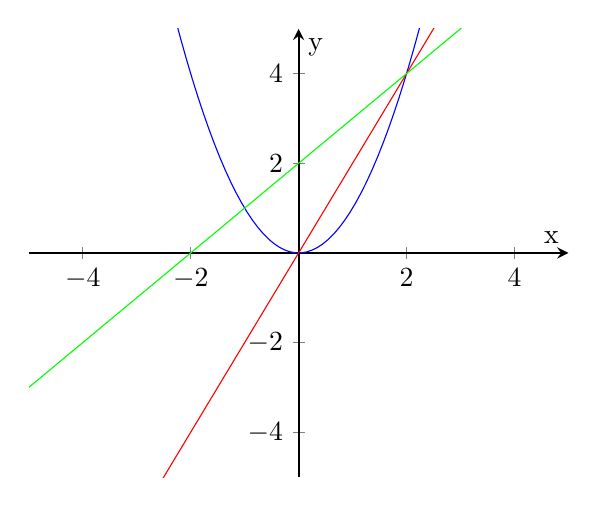
\begin{tikzpicture}
\begin{axis}[
    axis lines = middle,
    axis line style = thick,
    xmin = -5, xmax = 5,
    ymin = -5, ymax = 5,
    xlabel = x,
    ylabel = y
]
\addplot[
    domain = -5:5,
    samples = 100,
    color = blue
] {x^2};
\addplot[
    domain = -5:5,
    samples = 100,
    color = red
] {2*x};
\addplot[
    domain = -5:5,
    samples = 100,
    color = green
] {x + 2};
\end{axis}
\end{tikzpicture}
\end{center}
Word description: This graph shows three functions: $y = x^2$, $y = 2x$, and $y = x + 2$. We can see how the functions intersect and behave.

\begin{center}
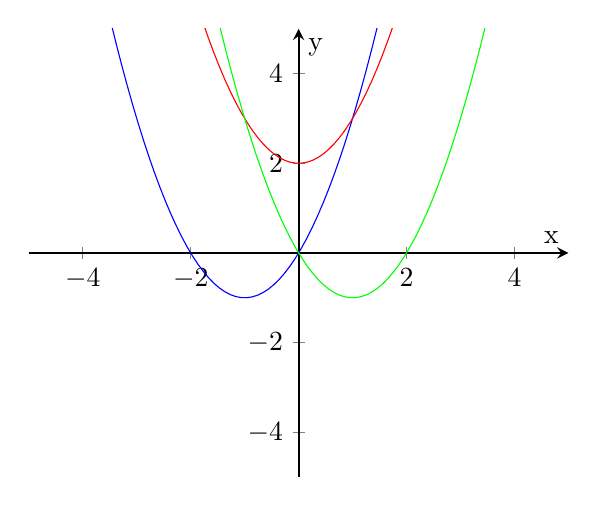
\begin{tikzpicture}
\begin{axis}[
    axis lines = middle,
    axis line style = thick,
    xmin = -5, xmax = 5,
    ymin = -5, ymax = 5,
    xlabel = x,
    ylabel = y
]
\addplot[
    domain = -5:5,
    samples = 100,
    color = blue
] {x^2 + 2*x};
\addplot[
    domain = -5:5,
    samples = 100,
    color = red
] {x^2 + 2};
\addplot[
    domain = -5:5,
    samples = 100,
    color = green
] {x^2 - 2*x};
\end{axis}
\end{tikzpicture}
\end{center}
Word description: This graph shows three functions: $y = x^2 + 2x$, $y = x^2 + 2$, and $y = x^2 - 2x$. We can see how the functions intersect and behave.

\begin{center}
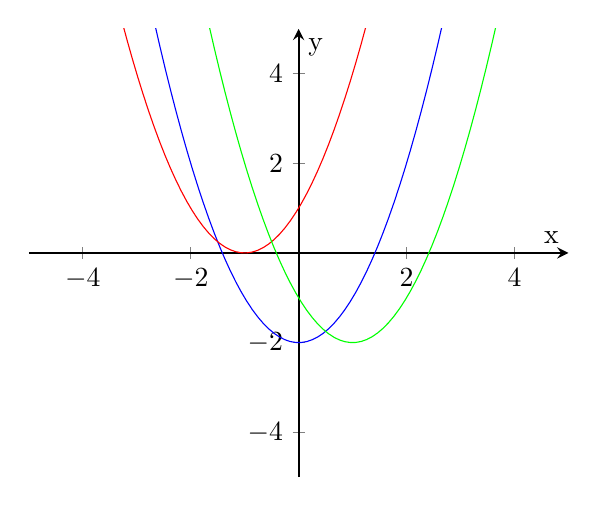
\begin{tikzpicture}
\begin{axis}[
    axis lines = middle,
    axis line style = thick,
    xmin = -5, xmax = 5,
    ymin = -5, ymax = 5,
    xlabel = x,
    ylabel = y
]
\addplot[
    domain = -5:5,
    samples = 100,
    color = blue
] {x^2 - 2};
\addplot[
    domain = -5:5,
    samples = 100,
    color = red
] {x^2 + 2*x + 1};
\addplot[
    domain = -5:5,
    samples = 100,
    color = green
] {x^2 - 2*x - 1};
\end{axis}
\end{tikzpicture}
\end{center}
Word description: This graph shows three functions: $y = x^2 - 2$, $y = x^2 + 2x + 1$, and $y = x^2 - 2x - 1$. We can see how the functions intersect and behave.

\section{Strategies and Procedures}
To simplify expressions, we can follow these steps:
\begin{itemize}
\item Combine like terms
\item Apply the distributive property
\item Apply the order of operations (PEMDAS)
\end{itemize}

Examples:
\begin{align*}
3x + 2x + 2 &= 5x + 2 \\
2(x + 3) &= 2x + 6 \\
\end{align*}

Subsection: Compare traditional vs. alternative approaches
\begin{itemize}
\item Traditional approach: Combine like terms first, then apply the distributive property and order of operations.
\item Alternative approach: Apply the distributive property first, then combine like terms and apply the order of operations.
\end{itemize}

Common mistakes and misconceptions:
\begin{itemize}
\item Forgetting to combine like terms
\item Applying the distributive property incorrectly
\item Not following the order of operations
\end{itemize}

\section{Vocabulary Table}
\begin{center}
\begin{tabular}{|c|c|}
\hline Term & Definition \\
\hline Like terms & Terms that have the same variable(s) raised to the same power \\
\hline Distributive property & $a(b + c) = ab + ac$ \\
\hline Order of operations & PEMDAS \\
\hline Expression & A combination of variables, constants, and mathematical operations \\
\hline
\end{tabular}
\end{center}

\section{Historical Context}
The concept of simplifying expressions dates back to ancient civilizations, where mathematicians used algebraic methods to solve problems. The modern notation and rules for simplifying expressions were developed in the 16th century.

Fun Facts \& Trivia:
\begin{itemize}
\item The word "algebra" comes from the Arabic word "al-jabr", meaning "reunion of broken parts".
\item The concept of simplifying expressions appears in movies, books, and art, such as in the movie "The Imitation Game" and in the book "The Da Vinci Code".
\end{itemize}

\section{Real-World Applications}
Simplifying expressions has many real-world applications:
\begin{itemize}
\item Financial applications: Simplifying expressions can help us calculate interest rates, investment returns, and costs.
\item Scientific applications: Simplifying expressions can help us model population growth, chemical reactions, and physical systems.
\item Biological applications: Simplifying expressions can help us model the spread of diseases, population dynamics, and genetic inheritance.
\end{itemize}

Example problems:
\begin{align*}
2x + 5x + 2 &= \\
3(x + 2) - 2x &= \\
\end{align*}

\section{Initial Explanation}
Simplifying expressions is a fundamental concept in algebra that involves combining like terms, applying the distributive property, and following the order of operations.

\section{Examples and Demonstrations}
Here are some examples and demonstrations of simplifying expressions:
\begin{align*}
3x + 2x + 2 &= 5x + 2 \\
2(x + 3) &= 2x + 6 \\
\end{align*}

\section{Applications Activity}
Simplifying expressions can be applied to real-world problems, such as:
\begin{itemize}
\item Calculating the cost of goods and services
\item Modeling population growth and decline
\item Analyzing scientific data and experiments
\end{itemize}

\section{Common Misconceptions Table}
\begin{center}
\begin{tabular}{|c|c|}
\hline Misconception & Correction \\
\hline Forgetting to combine like terms & Always combine like terms first \\
\hline Applying the distributive property incorrectly & Apply the distributive property correctly: $a(b + c) = ab + ac$ \\
\hline Not following the order of operations & Always follow the order of operations: PEMDAS \\
\hline
\end{tabular}
\end{center}

\section{Assessment Strategies}
To assess understanding of simplifying expressions, we can use:
\begin{itemize}
\item Quizzes and tests
\item Problem-solving activities
\item Projects and presentations
\item Hands-on activities, such as creating algebraic models and solving real-world problems
\end{itemize}

\section{Additional Resources}
For additional resources and support, we can use:
\begin{itemize}
\item Online tutorials and videos
\item Textbooks and workbooks
\item Algebraic software and calculators
\item Online forums and discussion groups
\end{itemize}

\section{Rationales}
The steps for simplifying expressions work because:
\begin{itemize}
\item Combining like terms allows us to simplify the expression by adding or subtracting like terms.
\item Applying the distributive property allows us to expand and simplify expressions.
\item Following the order of operations ensures that we perform mathematical operations in the correct order.
\end{itemize}

\section{Comparison Table}
\begin{center}
\begin{tabular}{|c|c|c|c|}
\hline Method & Efficiency & Accuracy & Applicability \\
\hline Traditional approach & Medium & High & General \\
\hline Alternative approach & High & Medium & Specific \\
\hline
\end{tabular}
\end{center}

\section{Practice Problems solved step by step}
Here are some practice problems solved step by step:
\begin{align*}
3x + 2x + 2 &= 5x + 2 \\
2(x + 3) &= 2x + 6 \\
\end{align*}

\section{Practice Problems}
Here are some practice problems for you to try:
\begin{align*}
2x + 5x + 2 &= \\
3(x + 2) - 2x &= \\
x^2 + 2x + 1 &= \\
x^2 - 2x - 1 &= \\
2x^2 + 3x - 2 &= \\
x^2 + 2x - 3 &= \\
3x^2 - 2x - 1 &= \\
2x^2 + x - 2 &= \\
x^2 - x - 2 &= \\
\end{align*}

Answers:
\begin{align*}
2x + 5x + 2 &= 7x + 2 \\
3(x + 2) - 2x &= 3x + 6 - 2x = x + 6 \\
x^2 + 2x + 1 &= (x + 1)^2 \\
x^2 - 2x - 1 &= (x - 1)^2 - 2 \\
2x^2 + 3x - 2 &= (2x - 1)(x + 2) \\
x^2 + 2x - 3 &= (x + 3)(x - 1) \\
3x^2 - 2x - 1 &= (3x + 1)(x - 1) \\
2x^2 + x - 2 &= (2x - 1)(x + 2) \\
x^2 - x - 2 &= (x - 2)(x + 1) \\
\end{align*}

\end{document}